\documentclass{article}
\usepackage{amsmath}
\usepackage[utf8]{inputenc}
\usepackage{float}
\usepackage{epsfig,graphicx}
\usepackage{xcolor,import}
\usepackage[german]{babel}
\usepackage{textcomp}
\usepackage{mathtools}

\begin{document}
\thispagestyle{empty}
			\begin{center}
			\Large{Fakultät für Physik}\\
			\end{center}
\begin{verbatim}


\end{verbatim}
							%Eintrag des Wintersemesters
			\begin{center}
			\textbf{\LARGE WINTERSEMESTER 2014/15}
			\end{center}
\begin{verbatim}


\end{verbatim}
			\begin{center}
			\textbf{\LARGE{Physikalisches Praktikum 1}}
			\end{center}
\begin{verbatim}




\end{verbatim}

			\begin{center}
			\textbf{\LARGE{PROTOKOLL}}
			\end{center}
			
\begin{verbatim}





\end{verbatim}

			\begin{flushleft}
			\textbf{\Large{Experiment Nr.8:} Wellenoptik}\\
							%Experiment Nr. und Titel statt den Punkten eintragen
			\LARGE{}	
			\end{flushleft}

\begin{verbatim}

\end{verbatim}	
							%Eintragen des Abgabedatums, oder des Erstelldatums des Protokolls
			\begin{flushleft}
			\textbf{\Large{Datum:}} \Large{05.12.2014}
			\end{flushleft}
			
\begin{verbatim}
\end{verbatim}
							%Namen der Protokollschreiber
		\begin{flushleft}
			\textbf{\Large{Namen:}} \Large{Veronika Bachleitner, Erik Grafendorfer}
			\end{flushleft}

\begin{verbatim}


\end{verbatim}
							%Kurstag und Gruppennummer, zb. Fr/5
			\begin{flushleft}
			\textbf{\Large{Kurstag/Gruppe:}} \Large{Fr/1}
			\end{flushleft}

\begin{verbatim}






\end{verbatim}
							%Name des Betreuers, das Praktikum betreute.
			\begin{flushleft}
			\LARGE{\textbf{Betreuer:}}	\Large{SCHAFLER}	
			\end{flushleft}
\newpage	

\section{Beugung am Spalt und Doppelspalt}

\subsection{Aufgabenstellung}
Wir vermessen das Beugungsbild hinter einem mit monochromatischem Licht  beleuchteten Einzelspalt und einem Doppelspalt. \\
Daraus berechnen wir die Spaltbreiten und den Spaltabstand.
\subsection{Grundlagen}
Trifft eine Welle auf ein Hindernis, wird jeder Punkt am Hindernis zum Ausgangspunkt einer neuen Welle; das ist das Huygensche Prinzip. Entstehen nah aneinander mehere neue Wellen, können diese miteinander interferieren. Dadurch werden sie gebeugt. Es gibt zwei Extremfälle der Beugung, die von der Beschaffenheit der Lichtquelle abhängen: Ist sie eine divergente Punktquelle, tritt Fresnelbeugung auf. Handelt es sich aber um annähernd parallele, etwa aus großer Ferne auftreffende Lichtstrahlen, tritt Fraunhoferbeugung auf. \\ 
Da wir in diesem Fall einen Laser verwenden beobachten wir Fraunhoferbeugung.\\
Um die Spaltbreite a zu erhalten verwenden wir folgende Beziehung, wobei n die Beugungsordnung des Minimums, $\lambda$ die Wellenlänge des verwendeten Lichts und $\alpha_n$ den Winkel, unter dem das Minimum zum Spalt beobachtet wurde, bedeuten:
\begin{equation}
\label{spaltbreite}
n\lambda=a sin(\alpha_n)
\end{equation}
Zur Berechnung von b, dem Spaltabstand am Doppelspalt, setzen wir folgende Formeln gleich:\\
$$sin(\alpha_{min,k})=\frac{\lambda}{2b}(2k+1)$$
$$sin(\alpha_{min,n})=\frac{n\lambda}{a}$$
Daraus erhalten wir für b:
\begin{equation}
\label{spaltabstand}
b=\frac{\lambda a}{2n\lambda}(2k+1)=\frac{a(2k+1)}{2n}
\end{equation}
\subsection{Versuchsaufbau und Methoden}
 Ein Laserstrahl trifft im ersten Versuchsteil auf einen Einzelspalt und im zweiten Teil auf einen Doppelspalt. Auf einem Schirm dahinter werden Beugungsbilder beobachtet. Aus den Distanzen der Minimia in den Beugungsbildern, sowie aus der Anzahl der Subminima können wir mit Kenntnis der Wellenlänge des verwendeten Lichtes auf die Beschaffenheit der Spalten schließen. 
\subsection{Durchführung}
Wir verwenden einen He-Ne-Laser (Wellenlänge = 632.8nm, Strahldivergenz = 1.2 mrad) der auf einer mit Längenmarkierungen versehenen Schiene (Genauigkeit $\pm 0.5mm$) ruht. Vor ihm platzieren wir erst einen Einzelspalt, später statt ihm einen Doppelspalt Auf einem Blatt Papier, das auf einem Schirm fixiert ist, der ebenfalls auf der markierten Schiene ruht, beobachten wir die Beugungsbilder. Auf diesem Blatt markieren wir die Minima mit Bleistift und messen dann die Abstände der Markierungen mit einer Schublehre (Genauigkeit $\pm$ 0.05 mm.) 
\subsection{Ergebnisse}
\textbf{Einzelspalt:}\\
\\
Wir bestimmen den Winkel zu den Minima $\alpha_n \approx \frac{d}{D}$, wobei d der Abstand der Minima vom Nullpunkt und D der Abstand des Spalts vom Schirm bedeuten und wir verwenden, dass für kleine Winkel der Tangens des Winkels annähernd dem Winkel ist. Hier ist $D=(1019 \pm 0.5)$\\

\begin{tabular}{|r|l|l|}
\hline
n & d & $\alpha_n$\\
\hline
1 & 5.70mm & 0.0056\\
2 & 11.35mm & 0.0111\\
3 & 17.55mm & 0.0172\\
4 & 22.90mm & 0.0225\\
5 & 28.30mm & 0.0278\\
\hline
\end{tabular}
\vspace{0.8cm}

Wir lassen uns a mithilfe einer linearen Regression in QTI-Plot berechnen:\\
Dabei wird die Formel $Y=AX+B$ verwendet, wobei bei uns $Y=n\lambda$, $X=sin(\alpha_n)\approx\frac{d}{D}$ und A die gesuchte Spaltbreite.\\

Daraus die Spaltbreite: 
$$\boxed{a=0.1140 \pm 0.0018mm}$$\\
\begin{center}
\begin{figure}
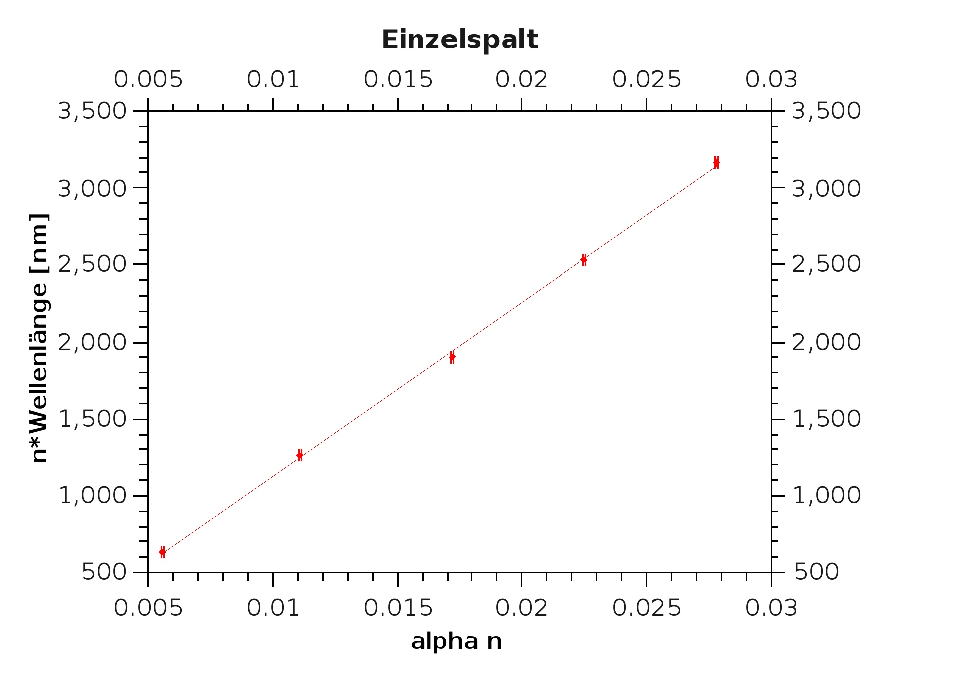
\includegraphics[scale=0.7]{einzelspalt.eps}
\end{figure}
\end{center}
\textbf{Doppelspalt:}\\
\\
Distanz der Minima vom Nullpunkt:\\
$\alpha_n=\frac{d}{D}$, wobei d der Abstand der Minima vom Nullpunkt und D der Abstand des Spalts vom Schirm. Hier ist $D=1000mm$\\
\begin{tabular}{|r|l|l|}
\hline
n & d & $\alpha_n$\\
\hline
1 & 5.30mm & 0.0053\\
2 & 10.90mm & 0.0109\\
3 & 16.15mm & 0.0162\\
4 & 21.10mm & 0.0211\\
\hline
\end{tabular}
\vspace{0.8cm}
\\Lassen die Spaltbreite a wieder von QTI-Plot berechnen:\\
\\
Also ist die Spaltbreite
$$\boxed{a=0.1200 \pm 0.0024 mm}$$
\\
Zur Berechnung von b setzen wir in (\ref{spaltabstand}) k=4, da wir im Hauptmaximum 8 Subminima gezählt haben, ein und erhalten:
$$b=\frac{a(2k+1)}{2n}=\frac{9a}{2}$$
$$\boxed{b=0.540 \pm 0.011 mm}$$
\begin{center}
\begin{figure}[H]
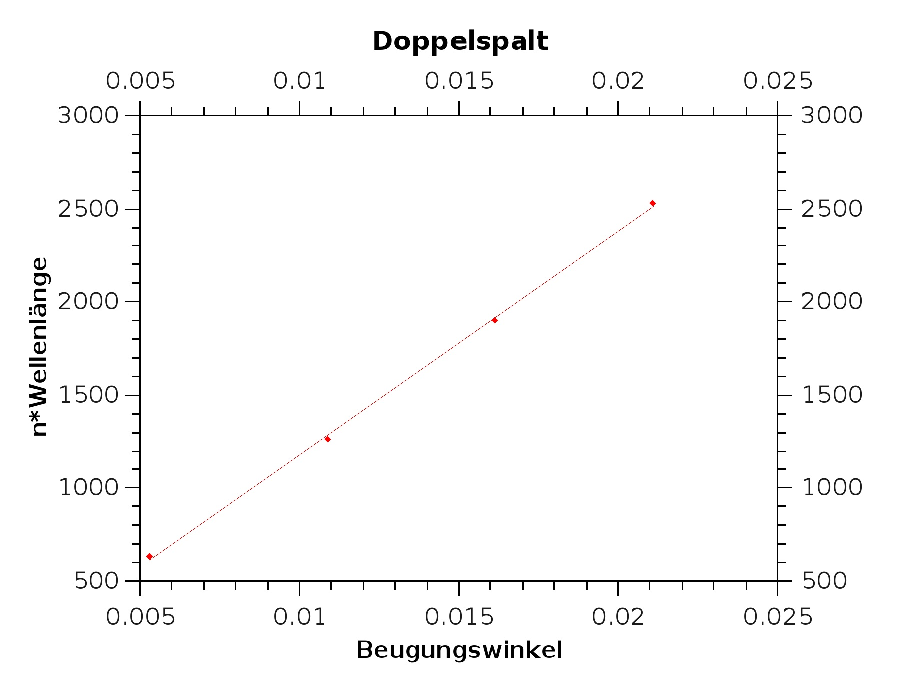
\includegraphics[scale=0.7]{doppelspalt.eps} 
\end{figure}
\end{center}
\section{Wellenlängenmessung mit dem Gitter}

\subsection{Aufgabenstellung}
Wir vermessen das Beugungsbild eines durch eine Spektrallampe beleuchteten Beugungsgitters. Wir bestimmen daraus Wellenlänge für die drei Spektrallinien und vergleichen unser Ergebnis mit den Literaturwerten.
\subsection{Grundlagen}
Wir beobachten wieder Fraunhoferbeugung. Hier entstehen durch die nah aneinander gelegenen Spalten im Gitter allerdings sehr viele neue Wellen, die miteinander interferieren und Beugung bewirken. Zusätzlich treten Nebenmaxima und Nebenminima auf indem Wellen von weiter entfernt liegenden Spalten sich gegenseitig verstärken und auslöschen. \\
Die Beziehung zwischen Wellenlänge, Gitterkonstante, Beugungsordnung und Beugungswinkel lautet \\
\begin{equation}
\label{gitter}
\lambda=\frac{sin(\vartheta)d}{n}
\end{equation}
\subsection{Versuchsaufbau und Methoden}
Wir haben eine Metalldampflampe, deren Licht auf ein Gitter mit der Gitterkonstante $10^{-5}$, das entspricht hunderttausend Gitterstäben pro Meter, fällt. Dieses Gitter ist fix auf einem Tisch plaziert, um den wir ein Teleskop rotieren, durch das wir die gebeugten Spektrallinien beobachten. Verschiedene Wellenlängen werden verschieden stark am Gitter gebegut. Wir messen die Rotationswinkel des Teleskops zu den jeweiligen Spektrallinien und berechnen uns mit ihnen die Wellenlängen der Linien, woraus wir auf die elementare Beschaffenheit des verwendeten Metallgases schließen können.
\subsection{Durchführung}

Der rotierende Teleskoptisch verfügt über ein Goniometer mit Nonius. Dadurch können wir auf Gradminuten genau messen.

\subsection{Ergebnisse}
Gitterkonstante: $d=10^{-5}$\\
Mit (\ref{gitter}) berechnen wir in der letzten Spalte die Wellenlängen:
\begin{center}
\begin{tabular}{|r|r|l|l|}
\hline
& Beugungsordnung & Halber Winkel & $\lambda$\\
\hline
\hline
blau & & &\\
& 1 & 2°30' & (436 $\pm$ 3)nm\\
& 2 & 4°58' & (433 $\pm$ 2)nm\\
& 3 & 7°32' & (436 $\pm$ 2)nm\\
\hline
grün & & &\\
& 1 & 3°4' & (535 $\pm$ 3)nm\\
& 2 & 6°16' & (546 $\pm$ 2)nm\\
& 3 & 9°23' & (543 $\pm$ 2)nm\\
\hline
gelb & & &\\
& 1 & 3°18' & (576 $\pm$ 3)nm\\
& 2 & 6°39' & (579 $\pm$ 2)nm\\
& 3 & 10°0' & (579 $\pm$ 1)nm\\
\hline
\end{tabular}
\end{center}
\vspace{0.8cm}

Daraus berechnen wir die gemittelten Wellenlängen:\\
blau: (435 $\pm$ 3)nm\\
grün: (541 $\pm$ 3)nm\\
gelb: (578 $\pm$ 3)nm\\

\subsection{Diskussion}
Es handelt sich höchstwahrscheinlich um ein Hg-Emissionsspektrum.\\
\\
Wenn wir die 
Literaturwerte für eine Hg-Lampe:\\
435.84 nm bzw. 434.75 nm bzw. 433.92 für blau\\
546.07 nm für grün\\
576.96 nm bzw. 579.07 nm für gelb\\
\\
mit unseren gemessenen Werten vergleichen, liegen zwei von drei sogar genau aufeinander, und einer, der für den grünen Anteil, leider nicht ganz im Vertrauensbereich, aber in Anbetracht der drei Messungen für diesen Wert von 535, 543 und 546 können wir annehmen, dass wir bei 535 ungenau gemessen haben. Wäre dieser Wert ein wenig höher, kämen wir mit gut in den Vertrauensbereich für den grünen Anteil einer Quecksilberdampflampe. Wir nehmen an, dass die kleine Noniusskala auf dem Goniometer unsere schwachen Augen überfordert hat.


\section{Newtonsche Ringe}

\subsection{Aufgabenstellung}
Wir projizieren Newtonsche Farbringe auf einen Schirm. Wir messen den Abstand der hellen und dunklen Zonen der Ringe und bestimmen daraus den Krümmungsradius der verwendeten Plankonvexlinse.
\subsection{Grundlagen}
Durch die nah aneinander laufenden Wellenzüge in der Konvexlinse und der Glasplatte können die leicht phasenverschobenen Wellen interferieren und so manche Farben verstärken, manche auslöschen. So entstehen die beobachteten Farbringe. \\
Zwischen den Radien der Farbringe und dem Krümmungsradius der Linse und der Wellenlänge des verwendeten Lichtes bestehen Beziehungen:
Für die dunklen Zonen beim reflektierten Gang gilt folgende Beziehung:
\begin{equation}
\label{reflexionradius}
r_k^2=R\cdot k\lambda
\end{equation}
Wobei $r_k$ den Radius des Farbringes bei k-ter Ordnung entspricht, und R dem Krümmungsradius der Linse.
Für die dunklen Zonen des transmittierten Lichtes gilt:
\begin{equation}
\label{transradius}
r_k^2=(2k-1)R\frac{\lambda}{2}
\end{equation}
\subsection{Versuchsaufbau und Methoden} Wir verwenden einen Aufbau aus einer Glühlampe und Linsen, die ihr Licht kollimieren und es auf eine plankonvexe Linse brechen, die sehr nahe auf einer planparellelen Platte liegt. Dabei verwenden wir eine Plankonvexlinse mit sehr großem Krümmungsradius. Durch die unterschiedlichen Wege, die das Licht durch diese Vorrichtung nimmt, interferieren die nahe aneinander laufenden Wellenzüge und erzeugen das Phänomen der Farbringe. Diese projizieren wir einmal nach einem direkten Durchgang durch die planparallele Platte, nach der Transmission, und einmal nach einer Reflexion an dieser Platte und einem erneuten Durchgang durch die konvexe Linse auf einen Schirm. 
\subsection{Durchführung}
Wir setzen einen Grünfilter vor die Lampe und erhalten dabei Licht mit einer Wellenlänge von (518 $\pm$ 3) nm. Die bunten Ringe werden zu klaren hellen und dunklen Ringen. Diese projizieren wir auf ein Blatt Papier auf einem Schirm - einmal aus Reflexion und einmal aus Transmission, nebeneinander. Dort markieren wir mit Bleistift die Mitten der dunklen Zonen. Mit einer Schublehre (Genauigkeit $\pm$ 0.05 mm) messen wir dann die Distanzen dieser Markierungen.
\subsection{Ergebnisse}
Das Bild bei der Reflexion ist in der Mitte dunkel; also berührt die konvexe Linse die Glasplatte. \\
Wellenlänge beim grünen Filter: $\lambda=(518 \pm 3)nm$

Die Newtonschen Ringe der Reflexion sind auf dem Schirm 2x vergrößert. Bei der Transmission sind sie 4x vergrößert.

$r_k$ bedeutet die Entfernung vom Nullpunkt bei k-ter Ordnung. Wir messen hier aber die Distanzen der Markierungen, also 2 mal $r_k$.\\
\begin{center}
\begin{tabular}{|c|c|}
\hline
\multicolumn{2}{|c|}{Reflexion, zweifache Vergrößerung} \\
\hline
Ordnung k & 2 $\cdot r_k$ \\
\hline
\hline
1 & 9.65 mm \\
2 & 13.75 mm  \\
3 & 16.45 mm\\
4 & 18.90 mm\\
5 & 21.55 mm\\
6 & 22.20 mm\\
\hline
\end{tabular}
\begin{tabular}{|c|c|}
\hline
\multicolumn{2}{|c|}{Transmission, vierfache Vergrößerung} \\
\hline
Ordnung k & 2 $\cdot r_k$ \\
\hline
\hline
1 & 24.65 mm \\
2 & 32.50 mm  \\
3 & 39.15 mm\\
4 & 44.55 mm\\
5 & 49.55 mm\\
6 & 53.85 mm\\
\hline
\end{tabular}
\end{center}
Mittels linearer Regression mit qti-plot gewinnen wir Werte für den Krümmungsradius der konvexen Linse:\\

\textbf{Reflexion}:

$$\boxed{ R_{refl}=(10 \pm 3)m }$$
\begin{center}
\begin{figure}
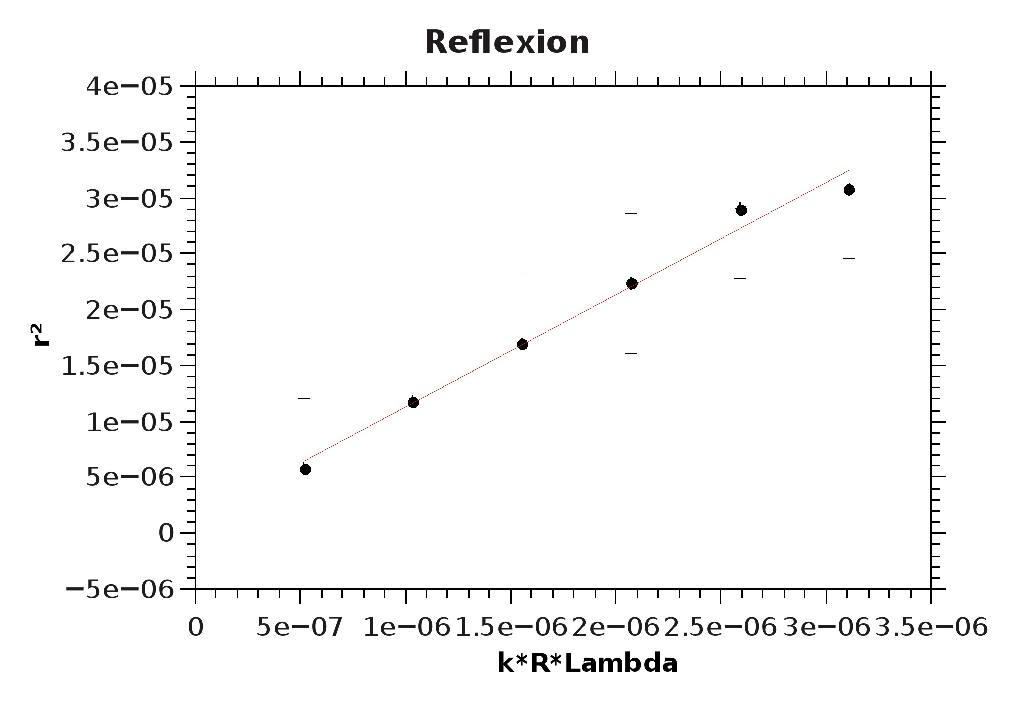
\includegraphics[scale=0.7]{refl.eps}
\end{figure}
\end{center}


\textbf{Transmission}:

$$\boxed{ R_{trans}=(14 \pm 3)m }$$
\begin{center}
\begin{figure}
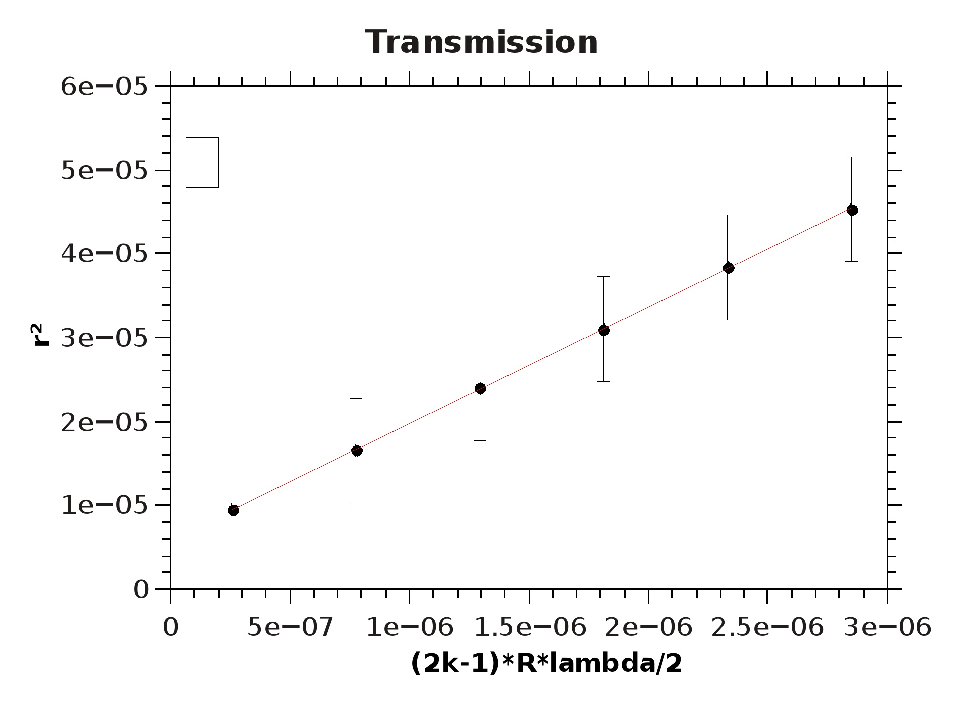
\includegraphics[scale=0.7]{trans.eps}
\end{figure}
\end{center}
\subsection{Diskussion}
Der als rund 13 Meter bekannte tatsächliche Krümmungsradius der Linse liegt in den Vertrauensbereichen unserer beiden Messungen; wir haben also wahrscheinlich genau gemessen. Auffallend ist, dass die Ungenauigkeit von $\pm$ 3 nm der Wellenlänge des Lichts durch den Filter kaum in die Ergebnisse eingeht, wie auch an den Plots zu sehen ist - hier sind die Fehlerbalken zwar prinzipiell einbezogen, aber unsichtbar klein. Die Unsicherheit der Messung mit der Schublehre geht dagegen sehr stark ein.\\
Zu erwähnen ist auch dass wir bei beiden Strahlengängen, bei der Reflexion und der Transmission, die dunklen Zonen gemessen haben. Wir haben deswegen aber bei der Transmission auch die entsprechende Formel zur Berechnung des Radius verwendet.
\end{document}
